\documentclass[crop=false]{standalone}
\usepackage{../imports}
\begin{document}
Quellenverweise:
\cite{DINISO9241112018}
\cite{hanssonEffectsPerformanceUsability2016}
\cite{DienstleistungenInformationstechnologieDeutschland}
Abkürzungen:
\ac{wia}
\\
Dies ist ein belangloser Fließtext. Dies ist ein belangloser Fließtext. Dies ist ein belangloser Fließtext. Dies ist ein belangloser Fließtext. Dies ist ein belangloser Fließtext. Dies ist ein belangloser Fließtext. Dies ist ein belangloser Fließtext. Dies ist ein belangloser Fließtext. Genauso belanglos wie die Test-Graphik \ref{figure:test} auf Seite \pageref{figure:test}. Richtig hübsch. Genauso wie die Beispiel-Tabelle \ref{table:beispiel} auf Seite \pageref{table:beispiel}. Auch nice. Oder die Formel \ref{equation:emc2} auf Seite \pageref{equation:emc2}. Alles sehr schön. Auch Verlinkungen auf andere Kapitel wie zum Beispiel Kapitel \ref{chapter:abstract} gehen.

\begin{wrapfigure}{r}{0.65\textwidth}
    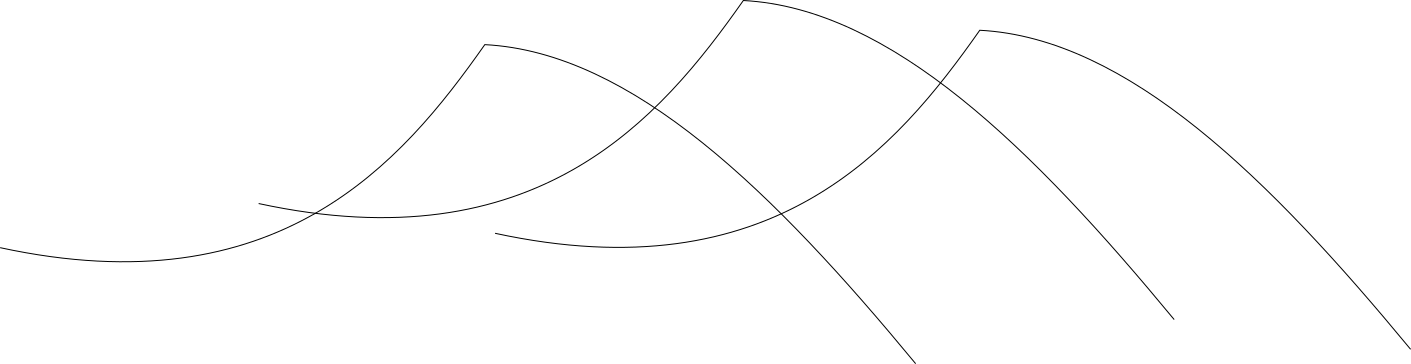
\includegraphics[width=0.63\textwidth]{example_graphic}
    \caption{Definitiv eine Vektor-Graphik. Weil die ja in Latex so angenehm sind. Will ich glatt als Hobby übernehmen so entspannt ist das, Vektor-Graphiken einzubinden.}
    \label{figure:test}
\end{wrapfigure}
Dies ist ein belangloser Fließtext. Dies ist ein belangloser Fließtext. Dies ist ein belangloser Fließtext. Dies ist ein belangloser Fließtext. Dies ist ein belangloser Fließtext. Dies ist ein belangloser Fließtext. Dies ist ein belangloser Fließtext. Dies ist ein belangloser Fließtext. 
Dies ist ein belangloser Fließtext. Dies ist ein belangloser Fließtext. Dies ist ein belangloser Fließtext. Dies ist ein belangloser Fließtext. 

\begin{wraptable}{l}{0.5\textwidth}
    \begin{longtable}{|l|l|l|}
        \hline
        Stadt   & Land     & Frucht  \\ \hline
        \endfirsthead
        %
        \endhead
        %
        Aachen  & Algerien & Apfel   \\ \hline
        Dresden & Dänemark & Dominik \\ \hline
    \end{longtable}
    \caption{Beispiel für eine Tabelle}
    \label{table:beispiel}
\end{wraptable}
Dies ist ein belangloser Fließtext. Dies ist ein belangloser Fließtext. Dies ist ein belangloser Fließtext. Dies ist ein belangloser Fließtext. Dies ist ein belangloser Fließtext. Dies ist ein belangloser Fließtext. Dies ist ein belangloser Fließtext. Dies ist ein belangloser Fließtext. 
Dies ist ein belangloser Fließtext. Dies ist ein belangloser Fließtext. Dies ist ein belangloser Fließtext. Dies ist ein belangloser Fließtext. 

\begin{wrapfigure}{r}{0.4\textwidth}
    \begin{equation}
        E=mc^2
    \end{equation}
    \caption{Eine sehr bekannte Formel}
    \label{equation:emc2}
\end{wrapfigure}
\Blindtext
\end{document}